\begin{figure}[t]
\centering
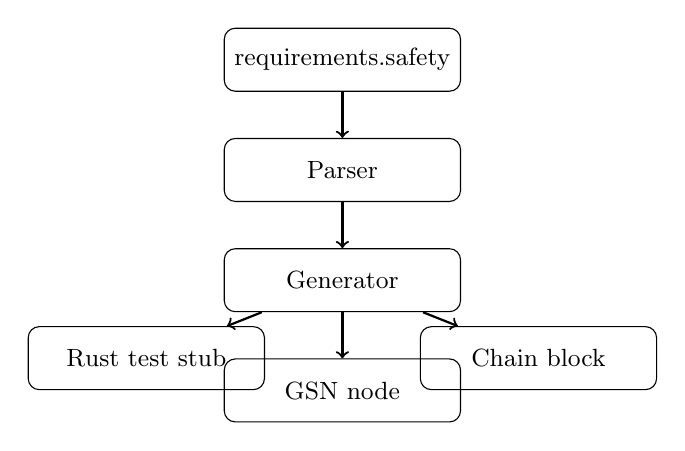
\begin{tikzpicture}[
    node distance=1.4cm,
    every node/.style={font=\small, draw, rectangle, rounded corners,
                        minimum width=3cm, minimum height=0.8cm, align=center}
]
\node (dsl) {requirements.safety};
\node (parse) [below of=dsl] {Parser};
\node (gen) [below of=parse] {Generator};
\node (test) [below left of=gen, xshift=-1.5cm] {Rust test stub};
\node (gsn) [below of=gen] {GSN node};
\node (chain) [below right of=gen, xshift=1.5cm] {Chain block};
\draw[->, thick] (dsl) -- (parse);
\draw[->, thick] (parse) -- (gen);
\draw[->, thick] (gen) -- (test);
\draw[->, thick] (gen) -- (gsn);
\draw[->, thick] (gen) -- (chain);
\end{tikzpicture}
\caption{SCC compilation pipeline. One requirements file generates three
artefacts, all derived from the same \texttt{Requirement} struct.}
\label{fig:scc-pipeline}
\end{figure}
